\documentclass[21pt, custom, portrait, plainboxedsections]{sciposter}

\setlength{\paperheight}{24in}
\setlength{\paperwidth}{48in}

\newcommand{\tabitem}{~~\llap{\textbullet}~~}
\definecolor{BoxCol}{RGB}{100, 155, 255}
\definecolor{charlesBlue}{RGB}{100, 155, 255}
\definecolor{SectionCol}{rgb}{1,1,1}

\usepackage[table, dvipsnames]{xcolor} 

\usepackage{epsfig}
\usepackage{amsmath}
\usepackage{amssymb}
\usepackage{multicol}
\usepackage{textcomp}
\usepackage[T1]{fontenc}
\usepackage[utopia]{mathdesign}
\usepackage{courier}

\usepackage{listings}
\lstset{breaklines}
\usepackage{subfig}
\usepackage{graphicx}
\usepackage[colorlinks=true,allcolors=charlesBlue]{hyperref}
\usepackage{siunitx}
\usepackage{setspace}
\usepackage{qrcode}

\usepackage{multirow}
\definecolor{LightCyan}{rgb}{0.88,1,1}

%%%%%%%%%%%%%%%%%%%%%%%%%%%%%%%%%
% environment for Stan code
\usepackage[T1]{fontenc} % needed for |
\usepackage{amsmath}
\usepackage{xspace}
\usepackage{fancyvrb}
\usepackage{url}
\usepackage{relsize} % defines \mathlarger
\DefineVerbatimEnvironment{stancode}{Verbatim}{fontsize=\small,xleftmargin=2em}

\usepackage{changepage}  % to adjust margins locally
\usepackage{wrapfig}  % wrap figure

\newtheorem{Def}{Definition}

\setmargins[4.5cm]

\renewcommand{\titlesize}{\fontsize{75}{20}}  %{\Huge} 
\renewcommand{\authorsize}{\fontsize{40}{20}} 
\renewcommand{\instsize}{\fontsize{30}{20}} 
\renewcommand{\sectionsize}{\Large}

\setlength{\columnseprule}{0.5pt}

% For customized tabular.
\newcolumntype{C}[1]{>{\centering\let\newline\\\arraybackslash\hspace{0pt}}m{#1}}
\newcolumntype{L}[1]{>{\raggedright\let\newline\\\arraybackslash\hspace{0pt}}m{#1}}

\title{
  \begin{flushleft} 
  \begin{adjustwidth}{-350pt}{100pt} \ \\
   Solving ODEs in a Bayesian context: challenges and opportunities
  \end{adjustwidth}
  \end{flushleft}
}

\rightlogo[0.5]{logo/stanLogo.png}  % same but on right

% to color column
\usepackage{colortbl}

\newcommand{\mc}[2]{\multicolumn{#1}{c}{#2}}
\definecolor{Gray}{gray}{0.95}

\newcolumntype{a}{>{\columncolor{Gray}}l}
\newcolumntype{b}{>{\columncolor{Gray}}c}
% \newcolumntype{b}{>{\columncolor{white}}c}

% Note: only give author names, not institute
\author{
  \begin{flushleft} 
  \hspace{-350pt} 
  \huge Charles C. Margossian$^\text{1}$, Lu Zhang$^\text{1}$, Sebastian Weber$^\text{2}$ and Andrew Gelman$^\text{1}$
  \large $^\text{1}$Department of Statistics, Columbia University, USA;
  $^\text{2}$Novartis Pharma, Switzerland.
  \end{flushleft}
} 
% insert correct institute name
%\institute{
%  \begin{flushleft}
%  \begin{adjustwidth}{-350pt}{0pt} 
%   \large $^\text{1}$Department of Statistics, Columbia University, USA;
%              $^\text{2}$Novartis Pharma, Switzerland.
%  \end{adjustwidth}
%  \end{flushleft}
%  }

% The following commands can be used to alter the default logo settings
%\leftlogo[1.1]{logo/ColumbiaMetrum}{  % defines logo to left of title (with scale factor)
%\rightlogo[0.9]{logo/stanLogo.png}  % same but on right



%%%%%%%%%%%%%%%%%%%%%%%%%%%%%%%%%%%%%%%%%%%%%%%%%%%%%%%%%%%%%%%%%%%%%%%%%%%%%%%%
%%% Begin of Document

\begin{document}
%define conference poster is presented at (appears as footer)

\conference{\Large Population Approach Group in Europe, September 2021}

\setlength{\fboxrule}{9pt}
\setlength{\fboxsep}{16pt}
\fcolorbox{charlesBlue}{white}{
\begin{minipage}{0.1in}
%\vspace*{4.8in}
%\vspace*{4\fontpointsize}
\end{minipage}
%\textcolor{white}{\maketitle}
\maketitle
%\textcolor{myDarkGreen}{\maketitle}
}

\begin{multicols}{3}
\raggedcolumns

\section*{Bayesian inference with Hamiltonian Monte Carlo}

\begin{figure}[H]
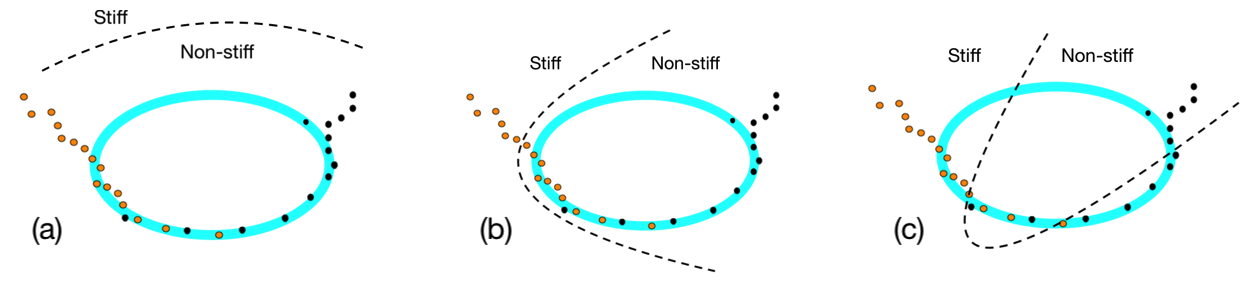
\includegraphics[width = 14in]{../figures/parameter_space_all}
\textbf{Figure 1.} \textit{As the Markov chains (orange and black dots) move across the parameter space, the behavior of the ODE may change. The elliptical blue band represents the sampling region, i.e. the region  where the posterior probability mass concentrates. Three hypothetical cases for how the ODE may behave.
%Hypothetical cases: (a) ODE is consistently non-stiff; (b) the orange chain starts in a stiff region but the ODE is non-stiff in the sampling region; (c) the ODE can either be stiff or non-stiff throughout the relevant regions.
}
\end{figure}

\textbf{Hamiltonian Monte Carlo.} Given observations, $y$, and parameters, $\theta$, our goal is to characterize the posterior distribution $p(\theta \mid y)$.
We focus on pharmacometrics models, for which the likelihood $p(y \mid \theta)$ uses an ODE.
\textit{Dynamic Hamiltonian Monte Carlo} (HMC) is a state-of-the-art Markov chains Monte Carlo method which draws approximate samples from $p(\theta \mid y)$ \cite{Betancourt:2018}.
Effective sampling crucially depends on properly tuning HMC's sampling parameters during a \textit{warmup phase}. \\

%\textbf{Bayesian models} are specified by a joint distribution over observations $y$ and latent variables $\theta$,
%$p(\theta, y) = p(y \mid \theta) p(\theta)$. In pharmacometrics, evaluating $p(y \mid \theta)$ often requires solving an ODE.
%\textit{Dynamic Hamiltonian Monte Carlo} (HMC) is a state-of-the-art Markov chains Monte Carlo method which draws approximate samples from $p(\theta \mid y)$ \cite{Betancourt:2018}.

%\begin{itemize}
%  \item[] \textbf{Bayesian models} are specified by a joint distribution over observations $y$ and latent variables $\theta$,
%$p(\theta, y) = p(y \mid \theta) p(\theta)$.
%  \item[] \textbf{Dynamic Hamiltonian Monte Carlo} (HMC) is a Markov chains Monte Carlo method which draws approximate samples from $p(\theta \mid y)$ and scales very well to high dimensions \cite{Betancourt:2018}. For HMC to sample effectively, 
%\end{itemize}

% HMC evaluates $\log p(\theta, y)$ and its gradient for many values of $\theta$ to efficiently explore the parameter space.
%\textbf{Trajectories in the parameter space.} HMC treats the chain as a ``physical particle'' imbued with a momentum $p$.
%We obtain a new iteration by simulating a physical trajectory according to Hamilton's equations of motion:
%\begin{equation*}
%  \frac{\text{d} \theta}{\text{d} t} = M^{-1} p; \ \ \ \ \ \frac{\text{d} p}{\text{d} t} = \nabla_\theta \log p(\theta, y),
%\end{equation*}
%%
%where $M$ is the \textit{mass matrix} or \textit{metric}.
%We solve this equation with a \textit{leapfrog integrator}, controlled by a step size $\epsilon$. \\

%\textbf{The tuning parameters of HMC} are:
%\begin{itemize}
%  \item $M^{-1}$: the inverse metric, which controls propensity to acceleration in various directions.
%  Usually we want to move more along directions that have a high posterior variance.
%  Hence we tune $M^{-1}$ using early estimates of the posterior covariance matrix. 
%  \item $\epsilon$: the integrator's step size, which trades speed and accuracy when solving the equations of motions. \\ 
%\end{itemize}
%\ \\
\textbf{Warmup phases of dynamic HMC} (e.g. for 500 iterations) \textbf{and prototype Path Finder.} \\
\begin{center}
  \begin{tabular}{b a | l}
   & \textbf{Adaptive HMC} & \textbf{Prototype Path finder} \\
  I & \tabitem starting at initialization, $\theta_0$, early exploration & \tabitem Construct optimization path between \\
  (75 iter) & \ \ \ \ with highly varying $\theta$. & \ \ \ \ $\theta_0$ and the mode of $p(\theta \mid y)$. \\
  & \tabitem convergence to sampling region. & \tabitem Find sampling region along path and \\
  & \tabitem initial tuning of the sampling parameters. & \ \ \ \ initialize HMC Phase I. \\
  \hline II & \tabitem semi-stable exploration of sampling region. & \tabitem Use variational approx. of $p(\theta \mid y)$ \\  
  (375 iter) & \tabitem more extensive tuning of sampling parameters, & \ \ \ \ to tune sampling parameters.  \\
   & \ \ \ \ as we learn more about $p(\theta \mid y)$. & \tabitem OR use Phase II of HMC.\\
  \hline III & \tabitem continued exploration of the sampling region. & \tabitem Use HMC's Phase III. \\ 
  (50 iter) & \tabitem final tuning of sampling parameters.
  \end{tabular}
\end{center} \ \\

\setlength{\columnseprule}{0pt}
\begin{multicols}{2}
\textbf{Challenge.} As $\theta$ changes, so can the behavior of the ODE in our model (Figure 1). \\

\textbf{Pathfinder \cite{Zhang:2021}.} The pathfinder offers alternative options for warming up HMC by (i) improving initialization
and (ii) estimating certain sampling parameters. (Figure 2)

\begin{center}
\textbf{Figure 2.}
\includegraphics[width = 4.5in]{../figures/pathfinder2}
\end{center}

\columnbreak

\end{multicols}


\columnbreak

\section*{Behavior of ODE-based models during HMC sampling}

\textbf{Michaelis-Menten PK model.} Consider a simple non-linear PK model:
\begin{multicols}{2}
\begin{eqnarray*}
  y_0' & = & - k_a y_0  \\
  y_1' & = & ka y_0 - \frac{V_m C}{K_m + C},
\end{eqnarray*}

\columnbreak

where $C = y_1 / V$ is the drug concentration in a central compartment.
The patient is administered a single dose and the drug concentration $c_\text{obs}$ is measured over time.
\end{multicols}
The full model, with parameters $\theta = \{k_a, V, V_m, K_m, \sigma\}$, is
\begin{eqnarray*}
  k_a \sim \text{logNormal}(\log(2.5), 3) ; \ \ \
  & V \sim \text{logNormal}(\log(35), 0.5); & \ \ \
  V_m \sim \text{logNormal}(\log(10), 0.5) ;  \\
  K_m \sim \text{logNormal}(\log(2.5), 3); \ \ \
  & \sigma \sim \text{Normal}^+(0, 1); & \ \ \
  c_\text{obs} \sim \text{Normal}(C, \sigma).
\end{eqnarray*}

\textbf{Which ODE integrator should we use?} \\

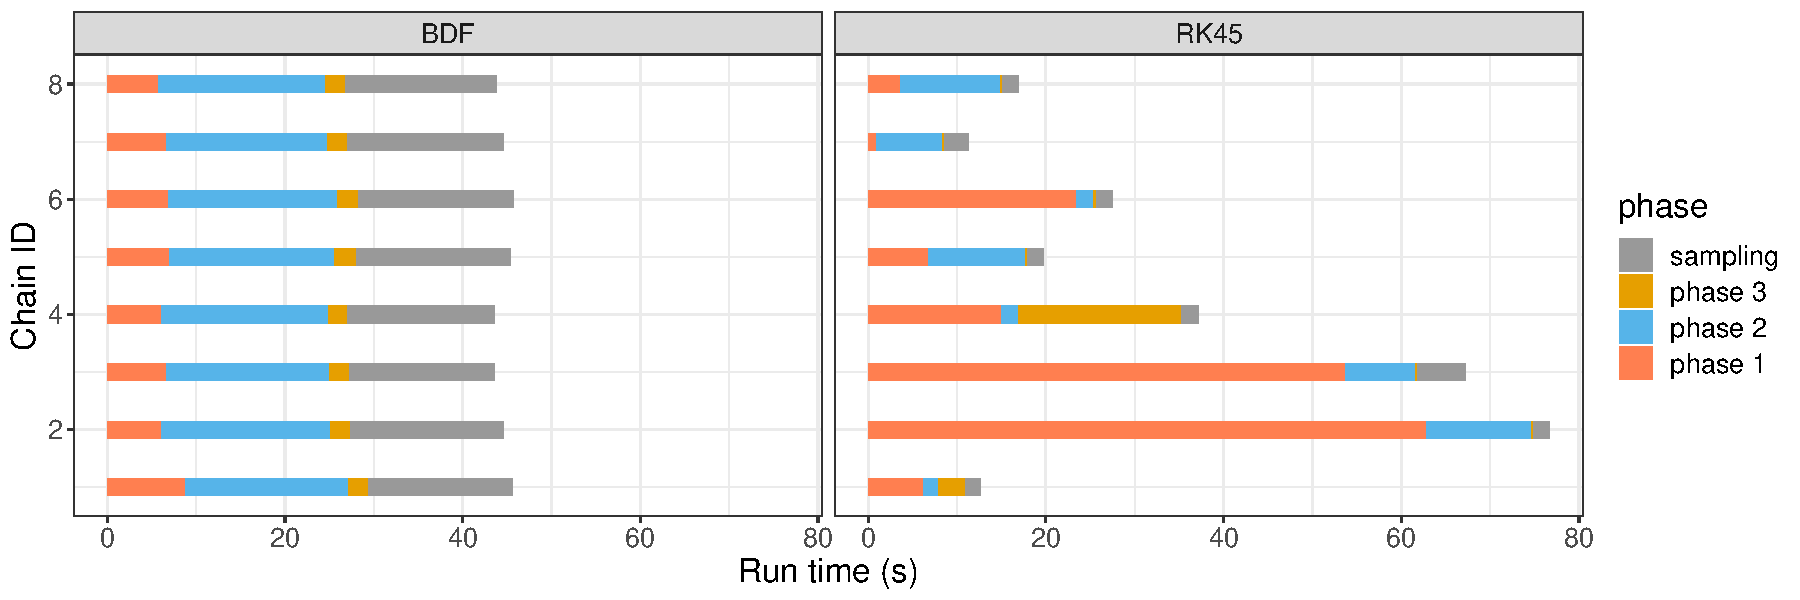
\includegraphics[width = 14.5in]{../figures/phase_time_facet_4x12.pdf}
\textbf{Figure 2.} \textit{Model runtimes using a stiff backward differentiation (BDF) integrator and a non-stiff Runge-Kutta $4^\text{th}/5^\text{th}$ (RK45) integrator.
For each integrator we run 8 HMC chains (500 warmup + 500 sampling iterations) using Stan \cite{Stan:2021}.} \\

%These results suggest no one integrator is optimal for all phases of HMC for this problem.
%RK45 is on average faster but very unstable, particularly during the early stages of warmup.
%Unfortunately, when running chains in parallel, the worst case informs the computational cost. \\

\textbf{Combining different integrators.} A robust integrator may be necessary during the warmup, but overkill when sampling.
Applying this heuristic, we propose the following schemes:

\begin{center}
\renewcommand{\arraystretch}{1.5}
\begin{tabular}{r c c c c c}
  & \textbf{Pathfinding} & \ \textbf{Phase I} \ & \ \textbf{Phase II} \ \ & \ \textbf{Phase III} \ & \ \textbf{Sampling} \ \\
  \textbf{HMC warmup, early switch} & NA & \cellcolor{Melon} BDF & \cellcolor{SkyBlue} RK45 & \cellcolor{SkyBlue} RK45 & \cellcolor{SkyBlue} RK45 \\
  \textbf{HMC warmup, late switch} & NA & \cellcolor{Melon} BDF & \cellcolor{Melon} BDF &  \cellcolor{SkyBlue} RK45 & \cellcolor{SkyBlue} RK45 \\
  \hline
  \textbf{Pathfinder, RK45} & \cellcolor{Melon} BDF  & \cellcolor{SkyBlue} RK45 & \cellcolor{SkyBlue} RK45 & \cellcolor{SkyBlue} RK45 & \cellcolor{SkyBlue} RK45 \\
  \textbf{Pathfinder, late switch} & \cellcolor{Melon} BDF & \cellcolor{Melon} BDF & \cellcolor{Melon} BDF & \cellcolor{SkyBlue} RK45 & \cellcolor{SkyBlue} RK45 \\
  \textbf{Pathfinder, approx. tuning} & \cellcolor{Melon} BDF & NA & NA & \cellcolor{SkyBlue} RK45 & \cellcolor{SkyBlue} RK45
\end{tabular}
\end{center}

\columnbreak

\section*{Performance Study}

We run all five proposed sampling schemes, as well as HMC using only RK45 or BDF on the Michaelis-Menten model and a population version of it.
The inference they produce are all in agreement. \\

\includegraphics[width = 12in]{../figures/performance_4x8.pdf} \\
\textbf{Figure 3.} \textit{Relaxation time, i.e. time to increase the effective sample size by 1, measured for $\log p(\theta, y)$. The orange crossed dot is the median time, and the red circled dot the worst time.
For method which run 8 or more chains in parallel,  we may prefer consistency to good median performance.} \\

\textbf{Model details.} The population model uses 3 patients, with partial pooling. 
We tried a centered and non-centered parameterization, and reported the former which for this particular problem produced more effective sampling.
We also found adapting a dense mass matrix for HMC worked better than using the default diagonal mass matrix.
The population uses 1,000 warmup and 1,000 sampling iterations. \\

\textbf{Results.}
\tabitem For the single patient model, using BDF during the warmup phase improves the stability of the sampler.
Improved initialization do not warrant the additional cost of running the pathfinder;
however estimating tuning parameters based on the variational approximation produces the most efficient sampler.
Improved implementation can further increase the benefits of the pathfinder.

\tabitem For the population model, we suspect the additional data stabilizes the posterior distribution, making uniform RK45 the best option.
For this model, running the pathfinder is expansive and the estimated tuning parameter is suboptimal
(we can diagnose this with the Pareto smooth importance sampling \cite{Zhang:2021}).


{\footnotesize
\bibliographystyle{abbrv}
\bibliography{BayesianODE}
}

% \end{tabular}
\end{multicols}



\end{document}

